\begin{figure}[t!]
    \centering
	    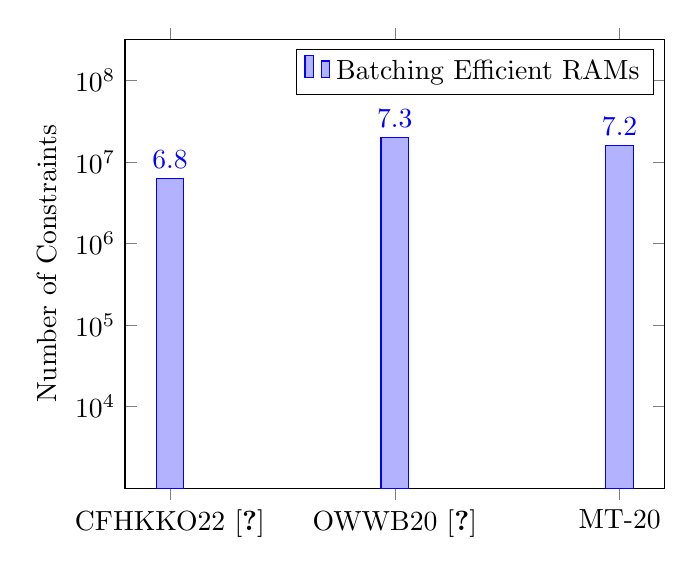
\begin{tikzpicture}
	        \begin{axis}[
	        ybar,
	        ylabel={Number of Constraints},
	        ymin = 3,
	        ymax = 8.5,
	        ytick = {4, 5, 6, 7, 8},
	        xlabel={},
	        xtick=data,
	        symbolic x coords= {A, B, C},
	        xticklabels = {CFHKKO22~\cite{CCS:CFHKKO22}, OWWB20~\cite{USENIX:OWWB20}, MT-20},
	        yticklabels = {$10^4$, $10^5$, $10^6$, $10^7$, $10^8$},
	        xlabel near ticks,
	        ylabel near ticks,
	        nodes near coords,
	        nodes near coords align={vertical},
	        ]
	        \addplot coordinates {(A,6.8) (B,7.3) (C,7.2)};
	        \legend{Batching Efficient RAMs}
	        \end{axis}
   	 \end{tikzpicture}
    \caption{Comparison of R1CS constraints incurred by existing approaches for batching efficient
    RAMs. MT20 refers to Merkle-tree with depth 20, instantiated using Poseidon hash.}
    \label{fig:batch-ram-constraints}
    \vspace*{-5mm}
\end{figure}

\begin{figure}[t!]
    \centering
	    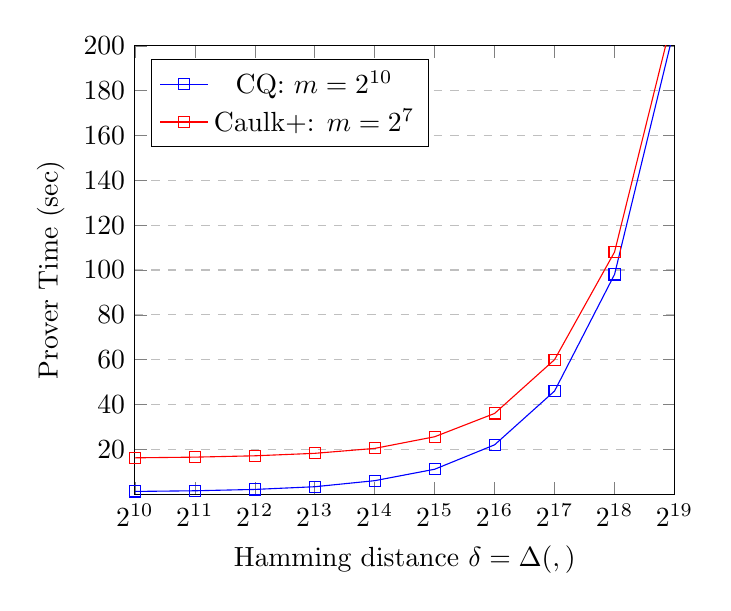
\begin{tikzpicture}
	        \begin{axis}[
	        xmin=0,
	        xmax=9,
	        ymin=0,
	        ymax=200,
	%		xlabel style={text width=0.5cm}, 
			xlabel= {Hamming distance $\delta = \Delta(\vecTbase,\vecT)$},
	        ylabel={Prover Time (sec)},
	        xtick={0, 1, 2, 3, 4, 5, 6, 7, 8, 9},
	        ytick={20, 40, 60, 80, 100, 120, 140, 160, 180, 200},
	        xticklabels={$2^{10}$, $2^{11}$, $2^{12}$, $2^{13}$, $2^{14}$, $2^{15}$, $2^{16}$, $2^{17}$, $2^{18}$, $2^{19}$},
	        yticklabels={20, 40, 60, 80, 100, 120, 140, 160, 180, 200},
	        legend pos=north west,
	        ymajorgrids=true,
	        grid style=dashed,
	        xlabel near ticks,
	        ylabel near ticks
	        ]
	        \addlegendimage{color=blue, mark=square}
	        \addlegendentry{CQ: $m=2^{10}$}
	        \addlegendimage{color=red, mark=square}
	        \addlegendentry{Caulk+: $m=2^{7}$}
	        \addplot[
	            color=blue,
	            mark=square,
	        ]
	        coordinates {
	            (0,1.2)(1,1.5)(2,2.1)(3,3.3)(4,6.0)(5,11.1)(6,22.0)(7,46)(8,98)(9,208)
	        };
	
	        \addplot[
	            color=red,
	            mark=square,
	        ]
	        coordinates {
	            (0,16.2)(1,16.5)(2,17.1)(3,18.2)(4,20.4)(5,25.6)(6,36)(7,60)(8,108)(9,216)
	        };
	        \end{axis}
	    \end{tikzpicture}
    \caption{Online proving time of updates on table $\vecT$ given the pre-processing parameters for table $\vecTbase$, plotted against the Hamming distance $\delta$ between $\vecTbase$ and $\vecT$. Here $m$ denotes the batch size of updates, while the RAM size is $N=2^{20}$. The blue plot corresponds to our scheme instantiated with CQ as the sub-vector argument (in a black-box manner). The red plot corresponds to the non-black-box adaptation of Caulk+ described in Appendix~\ref{app:committed-index-lookup}.}
    \label{fig:batch-ram-proving-time}
    \vspace*{-3mm}
\end{figure}

In this section we present a concrete evaluation of our batching efficient RAM and compare it to the
prior works on batching efficient RAM~\cite{USENIX:OWWB20,CCS:CFHKKO22}.
We also separately benchmark the effectiveness of our approach of computing encoded quotients presented
in Section~\ref{sec:update-protocol} over the na\"{i}ve approach.
 %on the experimental evaluation of our batching-efficient RAM.
%In addition, we also report on the overhead (as a function of changes since last parameter computation)
%incurred by our updatable lookup arguments over the vanilla lookup arguments with read-only table. We
%benchmark this overhead over vanilla implementations of Caulk+~\cite{EPRINT:PosKat22} and
%CQ~\cite{EPRINT:EagFioGab22}, both of which we also implement (as their non zero-knowledge variants)
%for our evaluation.
Our implementation is built on top of existing implementation~\cite{caulk-implementation}
of lookup argument Caulk~\cite{CCS:ZBKMNS22}. We make our implementation available at
\url{https://github.com/nitsatiisc/caulk/tree/updateable-ram}. 
%for anonymous submission. 
%We later plan to
%make the implementation available as open-source project.

\smallskip

\noindent{\bf Experimental Test-bed.} All the benchmarks were run single-threaded on a commodity configuration featuring a
$2.1GHz$ Intel-I5 processor, $16$ GB memory running Ubuntu Linux 22.04. The implementation was compiled using {\tt --release}
flag in Rust. Our protocol was instantiated for BLS12-381 curve, using the scheme CQ~\cite{EPRINT:EagFioGab22}
as the underlying sub-vector argument.

\smallskip

\noindent{\bf Online Proof Generation.} In Figure~\ref{fig:batch-ram-proving-time}, we benchmark the time
to prove a batch of $m=2^{10}$ updates on a table of size $N=2^{20}$. Here, the values on the $x$-axis denote
the hamming distance between the table on which the updates are being proved and the table whose pre-processed
parameters are used for the proof generation. Naturally, we expect the proving time to increase as the table
becomes more distant from the one used to generate pre-processed parameters. Our proof generation time stays
under a minute till the two table differ in almost $2\times 10^5$ positions. In conjunction with offline
pre-processing time from table~\ref{tbl:offline-proving-time}, the graph in Figure~\ref{fig:batch-ram-proving-time}
determines how the offline parameter generation should be scheduled to achieve optimal performance on average.

\smallskip

\noindent{\bf Offline Pre-Processing.} In Table~\ref{tbl:offline-proving-time} we provide the time to compute
table-specific parameters as a function of table size. This is the most computationally intensive step in our
scheme involving FFTs over group polynomials as the main bottle-neck. We believe offline pre-processing can be
made an order of magnitude more efficient by leveraging parallel implementation for the FFTs.

\begin{table}[htbp]
	\centering
    \begin{tabular}{|l|c|c|c|c|c|c|}
        \hline
        \cellcolor{lightgray} Table-Size ($N$) & $2^{10}$ & $2^{12}$ & $2^{14}$ & $2^{16}$ & $2^{18}$ & $2^{20}$ \\ \hline
        \cellcolor{lightgray} Time (s) & $7$ & $29$ & $135$ & $620$ & $2766$ & $12000$ \\ \hline
    \end{tabular}
    \caption{Pre-processing time for tables of different sizes.}
    \label{tbl:offline-proving-time}
%    \vspace*{-5mm}
\end{table}


\noindent{\bf Proof Size and Verification Costs.} Our proof sizes and verification costs are independent of the
size of the table and the number of updates in a batch. For the instantiation of our scheme with BLS12-381 curve,
we incur a proof size of $4.4KB$ while the verification takes around $15ms$.

\smallskip

\noindent{\bf Fast Update Benchmarks.} We also benchmark the efficiency of the algorithm to compute
 scalar coefficients in Lemma~\ref{lem:sum-computation}, required to assemble the encoded quotients from pre-computed quotients.
This algorithm is implemented and tested in the {\tt fastupdate} module of the referenced repository.
In Table~\ref{tbl:sum-computation-compare}, we compare it against the naive computation of the quotients.
In the table, we vary the sizes of set $I$ in Lemma~\ref{lem:sum-computation} in the set $\{2^i:7\leq i\leq 10\}$
and set $K=2^7|I|$. %i.e, we compare the two methods to sustain $\approx 100$ online proofs.
We clearly see $5\times-20\times$ advantage over the naive computation.

\smallskip

\noindent{\bf Continuity.} To maintain {\em continuity} of the system~(this is particularly important for applications such as rollups), we must carefully
align the online prover performance curve with the cost of offline computation.  As an example, suppose $\vec{T}_0$
is the initial pre-processed table at time $t=0$. We generate proofs using pre-computed parameters for $\vec{T}_0$
till the time $t=t_1$, when the table state $\vec{T}_1$ is at hamming distance $2^{17}$ from $\vec{T}_0$. At this point,
from Figure~\ref{fig:batch-ram-proving-time}, online proof generation takes around $40s$ for batch of $1000$ updates.
At $t=t_1$, we also start an offline parameter computation for the table $\vec{T}_1$, while continuing to generate
online proofs using parameters for $\vec{T}_0$. We can generate the next $2^7$ batches of updates at an average of
approximately $12000/128\approx 94s$ each, thus finishing with a table state $\vec{T}_2$ at hamming distance at most
$2^{18}$ from $\vec{T}_0$ at $t_2=t_1+12000$. At this point, we should have the pre-computed parameters for $\vec{T}_1$,
which is at update distance of $2^{17}$ from $\vec{T}_2$, and thus online proof generation can switch to parameters
for the table $\vec{T}_1$. This alignment gives us a proving time of $94s$ per batch of $1000$, while ensuring system
is live at all times. Clearly, a faster offline pre-computation using parallel implementation would allow us to stay
at the cheaper end of online proving performance.


\begin{table}[htbp]
    \centering
    \begin{tabularx}{0.45\textwidth}{@{}XXXX@{}}
        \toprule
        $|I|$ & $|K|$ & Lemma~\ref{lem:sum-computation} & Naive \\ \midrule
        $2^7$ & $2^{14}$ & 3.3s  & 12s \\
        $2^8$ & $2^{15}$ & 7.7s  & 48s \\
        $2^9$ & $2^{16}$ & 16.8s & 198s \\
        $2^{10}$ & $2^{17}$ & 39.2s & 839s \\
        \bottomrule
    \end{tabularx}
    \caption{Comparison of Lemma~\ref{lem:sum-computation} and naive computation for calculating
    scalar coefficients for encoded quotients.}
    \label{tbl:sum-computation-compare}
    \vspace*{-5mm}
\end{table}

\noindent{\bf Comparison with Prior Works}. The proof generation in the prior batching efficient RAM constructions
using RSA accumulators~\cite{USENIX:OWWB20,CCS:CFHKKO22} involves two key steps (i) generation of a SNARK
proof showing knowledge of witness for a relation modeled as arithmetic circuit/R1CS and (ii) computing the witness
for the proof generation. A platform agnostic metric to express the cost of the first step is the number of R1CS
constraints needed to encode the relation, which is also the metric used in~\cite{CCS:CFHKKO22} for comparison.
Using the R1CS constraints reported in~\cite{USENIX:OWWB20,CCS:CFHKKO22} (see Figure~\ref{fig:batch-ram-constraints}),
we benchmark single-threaded proof generation
using the \textsf{Groth16} protocol (used in prior works) for R1CS of equivalent size on our test-bed. We use publicly
available benchmarking suite in~\cite{ark-groth-16} for \textsf{Groth16} benchmarks. Since the
the prior works only report performance of parallel implementation of the second step which is common to both (with
degree of parallelism not explicitly mentioned), we will use the reported parallel performance to estimate the
overall proving time with this caveat. 

Even without the benefit of parallelization, our average proof generation
time of $\approx 90s$ for batch size of $2^{10}$ and RAM size of $2^{20}$ is $3-5\times$ faster than the prior works
for the same setting. The proof sizes and verification complexity are constant for prior work and our work.
Concrete proof sizes are smaller in~\cite{USENIX:OWWB20,CCS:CFHKKO22} owing to their usage of \textsf{Groth16}
proving backend, while our verification times are competitive with~\cite{USENIX:OWWB20} and substantially
less than~\cite{CCS:CFHKKO22}. One way to reduce proof size in our scheme would be to use a SNARK to prove
memory-checking on smaller sub-RAMs, instead of explicit polynomial protocol that we employ for the same. For
completeness, we also include the batching efficient RAM using Merkle tree (with Poseidon hash) in the performance
comparison in Table~\ref{tbl:performance-comparison} which was considered in prior works. Note that the Merkle
 tree-based approach is faster than that of~\cite{USENIX:OWWB20} for batch size of $2^{10}$ (the break-even
 point reported to be batch size of $\approx 1200$).

\begin{table}[htbp]
    \centering
    \begin{tabularx}{0.8\textwidth}{@{}XXXX@{}}
        \toprule
        Scheme & $\prover$ (s) & $\verifier$ (ms) & $|\pi|$ (KB) \\ \midrule
        MT20 & $450$ & $7$  & $0.26$ \\
        OWWB20~\cite{USENIX:OWWB20} & $550+43$ & $7$  & $0.26$ \\
        CFHKKO22~\cite{CCS:CFHKKO22} & $226+43$ & $120$ & $1.3$ \\
        Our Work & $94$ & $15$ & $4.4$ \\
        \bottomrule
    \end{tabularx}
    \caption{Comparing performance of our batching-efficient RAM with prior works. $\prover$
    denotes proof generation time, $\verifier$ denotes verification time while $|\pi|$ denotes
    argument size. We mention proof generation time as $a+b$ for~\cite{USENIX:OWWB20,CCS:CFHKKO22}
    where $a$ denote proving time of \textsf{Groth16} and $b$ denotes witness generation time. The latter
    is reported in respective works for a parallel implementation.}
    \label{tbl:performance-comparison}
    \vspace*{-5mm}
\end{table}


%Generating table specific parameters for table of size $1$ million takes around $12,000$
%seconds for CQ based instantiation.

%We first provide overall running time of batching-efficient RAM primitive instantiated with Caulk+
%and CQ lookup arguments. The degradation in running time is plotted as function of accumulated updates
%since the last computation of full table-specific parameters in Figure~\ref{fig:batch-ram-proving-time}.
%We choose batch size of $m=128$ for Caulk+ based instantiation (to avoid prohibitive performance),
%while we consider $m=1024$ for CQ based instantiation. Our overhead remains barely noticable against
%the quadratic costs incurred by Caulk+ base protocol till about $2^{15}$ accumulated changes, equivalent of
%$128$ lookups of size $512$. While the performance overhead compared to base CQ protocol is much more apparent,
%overall we continue to achieve online proof generation time of under a minute all the way upto
%$\approx 2\times 10^5$ accumulated changes, equivalent of roughly $200$ batch updates (assuming the worst-case
%scenario). In real application scenarios, we can expect better degradation curve, as its unlikely that updates
%to the table occur uniformly across all positions.

%In Figure~\ref{fig:batch-ram-constraints}, we compare the
%R1CS constraints incurred by existing approaches to batching friendly RAMs/accumulators. For our work, we assume
%that the memory checking on the RAM instance of size $m$ is implemented as an arithmetic circuit using a Bene's
%routing network~\cite{benes}, though we also provide a purely polynomial protocol for the same in Section~\ref{sec:poly-proto-ram-app}.
%Our construction is relatively ``circuit-free'' and relies on the efficiency of lookup arguments coupled with
%our novel modifications to make them update resilient.





